\documentclass[letterpaper,12pt,fleqn]{article}
\usepackage{matharticle}
\usepackage{siunitx}

\pagestyle{empty}

\begin{document}

\section*{Introduction}

There are some problems that algebra alone cannot solve:

\begin{enumerate}
\item The slope of a tangent line to a curve
\item The area under a curve
\item Infinite sequences
\item Infinite series
\end{enumerate}

\subsection*{Slope of a Tangent Line to a Curve}

\bigskip

\begin{definition}[Rate-of-change Problem]
  A \emph{rate-of-change} problem seeks to determine how much one quantity changes with respect to a change in
  another quantity.
\end{definition}

\begin{examples}[Rate-of-change Problems with respect to Time]
  \begin{itemize}[left=0in]
  \item[]
  \item The velocity (speed) of a moving object (miles per hour, feet per second).
  \item The rate at which a product is produced during a chemical reaction (grams per second).
  \item The rate of radioactive decay (grams per year).
  \item The rate of population growth (members per year).
  \item The rate of change in the price of a stock during a particular trading day (dollars per hour).
  \end{itemize}
\end{examples}

\begin{examples}[Rate-of-change Problems with respect to Other Quantities]
  \begin{itemize}[left=0in]
  \item[]
  \item The change in gravitational force applied to the earth with respect to changing distance from the sun
    (newtons per kilometer).
  \item The change in magnetic force applied to an iron nail with respect to changing distance from a magnet (newtons
    per centimeter).
  \item Elasticity of demand: the change in the quantity of a commodity sold with respect to a change in price
    (units per dollar).
  \end{itemize}
\end{examples}

Algebraically, these situations are modeled by a function \(y=f(x)\).  The quantity measured is represented by the
dependent variable \(y\) and the quantity causing the change is represented by the independent variable \(x\).
Note that the variable names can change to represent the actual quantities in the problem.  Furthermore, the
function name usually matches the independent variable name.

\newpage

\begin{example}

  The position \(s\) of a moving body with respect to time \(t\) is modeled by \(s=s(t)\):

  \bigskip

  \begin{center}
    \begin{tikzpicture}
      \draw [help lines,->] (0,0) -- (6,0) node [right] {\(t\)};
      \draw [help lines,->] (0,0) -- (0,4) node [above] {\(s\)};
      \draw [smooth,rounded corners=5mm]
      (0,2) .. controls (1,3) .. (2,3) .. controls (3,3) .. (4,1) .. controls (5,1) .. (6,3.5)
      node [above] {\(s(t)\)};
      \node [closed point] at (2,3) {};
      \draw [dashed] (2,3) -- (2,0);
      \node [below] at (2,0) {\(t_1\)};
      \node [closed point] at (3.5,2) {};
      \draw [dashed] (3.5,2) -- (3.5,0);
      \node [below] at (3.5,0) {\(t_2\)};
      \node [closed point] at (5.5,2.2) {};
      \draw [dashed] (5.5,2.2) -- (5.5,0);
      \node [below] at (5.5,0) {\(t_3\)};
      \draw [dashed] (2,3) -- (0,3);
      \node [left] at (0,3) {\(s(t_1)\)};
    \end{tikzpicture}
  \end{center}

  Determining the body's position \(s\) at some time \(t\) is easy: \(s(t_1)\).  However, how the position is
  changing at a particular time \(t\) is a completely different question:

  \bigskip

  \begin{center}
    \begin{tabular}{|c|c|}
      \hline
      time & position \\
      \hline
      \hline
      \(t_1\) & constant \\
      \hline
      \(t_2\) & decreasing \\
      \hline
      \(t_3\) & increasing \\
      \hline
    \end{tabular}
  \end{center}
\end{example}

The goal of rate-of-change problems is to quantify the magnitude of such changes.

This is easy when the model is linear: \(y=f(x)\) is a line.

\begin{example}
  Consider a body moving in a straight line at constant velocity \SI{0.75}{ft/sec} with initial position
  \(s(0)=\SI{2}{ft}\).  The equation of motion is given by:
  \[s(t)=\frac{3}{4}t+2\]
  \begin{center}
    \begin{tikzpicture}[scale=0.9]
      \begin{axis}[
          axis lines=middle,
          xmin=0,
          xmax=5,
          ymin=0,
          ymax=8,
          ticks=none,
          xlabel={\(t\)},
          ylabel={\(s\)},
          x label style={at={(axis cs:5,0)},anchor=west},
          y label style={at={(axis cs:0,8)},anchor=south},
          clip=false
        ]
        \addplot [domain=0:5,blue] {(3/4)*x+2} node [right] {\(s(t)=\frac{3}{4}t+2\)};
        \node [left] at (0,2) {\(s_0=2\)};
      \end{axis}
    \end{tikzpicture}
  \end{center}

  \bigskip

  The equation of motion is linear and the velocity is the slope of the line.

  From a unit analysis standpoint:
  \[\left(\frac{\si{ft}}{\si{sec}}\right)\si{sec}+\si{ft}=\si{ft}\]
  Thus, the change in position with respect to a change in time at any time \(t\) is simply the slope of the line.
  In fact, this is exactly how the slope of a line is calculated:
  \[v=\frac{\Delta s}{\Delta t}=\frac{s_2-s_1}{t_2-t_1}\]
\end{example}

But what happens when the function is not linear?

\begin{definition}[Rate-of-change of a Function at a Point]
  Let \(f(x)\) be a function.  The \emph{rate-of-change} of the the function at a point \((c,f(c))\) is the slope
  of the tangent line to the function at that point.
\end{definition}

We use this definition because it works.  In the above example, the tangent line at \((t_1,f(t_1))\) appears to be
horizontal (slope=0), indicating that the function is constant.  At \((t_2,f(t_2))\) the tangent has a negative
slope, indicating that the function is decreasing.  At \((t_3,f(t_3))\) the tangent has a positive slope, indicating
that the function is increasing.  Furthermore, the steeper the function, the steeper the tangent line.

Unfortunately, there is no way using just algebra to determine the slope of a tangent line to a general curve at a
point.

Why do we care?
\begin{enumerate}
\item Was a car exceeding a speed limit when it passed a checkpoint?
\item Which chemical reaction produces product the fastest?
\item Is a radioactive substance safe for humans?
\item Has a population's reproduction rate fallen beneath the replacement level?
\item Will an increase in the price of a product produce more revenue?
\end{enumerate}

\subsection*{Area Under a Curve}

\begin{definition}[Summation Problem]
  A \emph{summation problem} seeks to determine the accumulation of a changing quantity given a change in
  another quantity.
\end{definition}

For summation problems, a rate-of-change function \(f(x)\) and a region of the independent variable \(x\) are
given.

\begin{example}
  A car is traveling at a constant speed of \SI{60}{mph}.  How far does the car travel in \SI{2}{hours}?

  This is simply a distance equal rate times time problem:
  \[d=(\SI{60}{mi/hr})(\SI{2}{hr})=\SI{120}{mi}\]
  Interpreted geometrically:

  \bigskip

  \begin{center}
    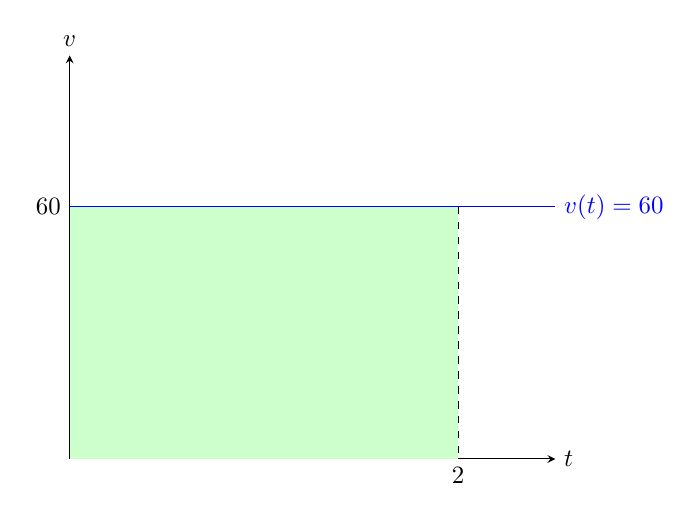
\begin{tikzpicture}[scale=0.9]
      \begin{axis}[
          axis lines=middle,
          xmin=0,
          xmax=5,
          ymin=0,
          ymax=8,
          ticks=none,
          xlabel={\(t\)},
          ylabel={\(v\)},
          x label style={at={(axis cs:5,0)},anchor=west},
          y label style={at={(axis cs:0,8)},anchor=south},
          clip=false
        ]
        \addplot [domain=0:5,blue] {5} node [right] {\(v(t)=60\)};
        \node [left] at (0,5) {\(60\)};
        \fill [green!20!white] (0,0) rectangle (4,5);
        \draw [dashed] (4,5) -- (4,0) node [below] {\(2\)};
      \end{axis}
    \end{tikzpicture}
  \end{center}

  \bigskip

  Note that the area under the rate-of-change curve in the selected region is calculated.
\end{example}

But what if the rate-of-change function is not constant?  The total is still the area under the curve.

\begin{example}
  A car is traveling with a speed that increases linearly from \SI{0}{mph} to \SI{60}{mph} after one hour, and then
  decreases linearly from \SI{60}{mph} to \SI{0}{mph} over the next hour.  How far does the car travel?

  \bigskip

  \begin{center}
    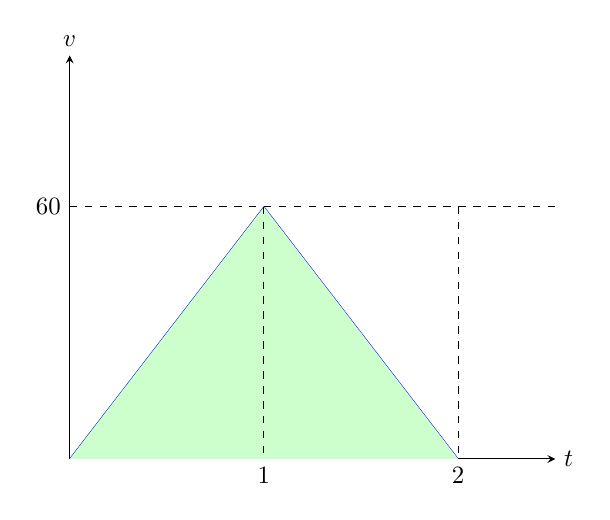
\begin{tikzpicture}[scale=0.9]
      \begin{axis}[
          axis lines=middle,
          xmin=0,
          xmax=5,
          ymin=0,
          ymax=8,
          ticks=none,
          xlabel={\(t\)},
          ylabel={\(v\)},
          x label style={at={(axis cs:5,0)},anchor=west},
          y label style={at={(axis cs:0,8)},anchor=south},
          clip=false
        ]
        \addplot [dashed,domain=0:5] {5};
        \addplot [domain=0:2,blue] {2.5*x};
        \addplot [domain=2:4,blue] {2.5*(4-x)};
        \node [left] at (0,5) {\(60\)};
        \fill [green!20!white] (0,0) -- (4,0) -- (2,5) -- cycle;
        \draw [dashed] (4,5) -- (4,0) node [below] {\(2\)};
        \draw [dashed] (2,5) -- (2,0) node [below] {\(1\)};
      \end{axis}
    \end{tikzpicture}
  \end{center}
  \[d=\frac{1}{2}(\SI{60}{mi/hr})(\SI{2}{hr})=\SI{60}{mi}\]
\end{example}

\subsection*{Infinite Sequences}

\subsection*{Infinite Series}

\end{document}
